\documentclass[10pt]{beamer}

% ------------------------------------------------------------------------
% Carga del preámbulo personalizado (preamble.tex)
% (Asegúrate de tenerlo en la misma carpeta para que \input funcione)
% ------------------------------------------------------------------------
\usetheme[progressbar=frametitle]{metropolis}
\usepackage{appendixnumberbeamer}
\usepackage{fancyvrb}
\usepackage{booktabs}
\usepackage[scale=2]{ccicons}
\usepackage{pgfplots}
\usepgfplotslibrary{dateplot}
\usepackage{type1cm}
\usepackage{lettrine}
\usepackage{ragged2e}
\usepackage{xspace}
\newcommand{\themename}{\textbf{\textsc{metropolis}}\xspace}
\usepackage{graphicx} % Allows including images
\usepackage{booktabs} % Allows the use of \toprule, \midrule and \bottomrule in tables
\usepackage[utf8]{inputenc} %solucion del problema de los acentos.
\usepackage{xcolor}
\definecolor{LightGray}{gray}{0.9}

\usepackage{minted}
\usemintedstyle{tango}
\newcommand{\mypyfile}[1]{\inputminted[linenos=true, fontsize=\footnotesize, frame=lines, framesep=5\fboxrule,framerule=1pt]{python}{#1}}

\setminted[python]{breaklines,frame=lines,framesep=2mm,baselinestretch=1.2,bgcolor=LightGray,linenos, fontsize=\footnotesize} % obeytabs=true, tabsize=2, showtabs=true}

%%%%%%%%%%%%%%%%%%%%%%%%%%%%%%%%%%%%%%%%%%%%%%%%%%%%%%%%%%%%%%%%%%%%%%%%%%%%%%%%%%%%%%
\setbeamercolor{progress bar}{fg=blue!50!black,bg=white!50!black}
\setbeamercolor{title separator}{fg=red!50!black,bg=white!50!black}
\setbeamercolor{frametitle}{fg=white!80!black,bg=red!50!black}
\title[PCFI161]{Programaci\'on para F\'isica y Astronom\'ia}
\subtitle{Departamento de Física.}

\newcommand{\myfront}{
\author[PCFI161]{Corodinadora: C Loyola \\ Profesoras/es C Loyola / C Femenías / Y Navarrete / C Ruiz}
\institute[UNAB]{Universidad Andrés Bello}
\date{Primer Semestre 2025}
}

\titlegraphic{%
  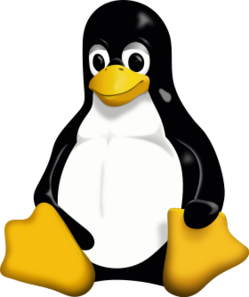
\includegraphics[width=.08\textwidth]{logo-tux.png}\hfill
  
\includegraphics[width=.3\textwidth]{logo-unab.png}\hfill
  
\includegraphics[width=.08\textwidth]{logo-python.png}
}

\makeatletter
\setbeamertemplate{title page}{
  \begin{minipage}[b][\paperheight]{\textwidth}
    \vfill%
    \ifx\inserttitle\@empty\else\usebeamertemplate*{title}\fi
    \ifx\insertsubtitle\@empty\else\usebeamertemplate*{subtitle}\fi
    \usebeamertemplate*{title separator}
    \ifx\beamer@shortauthor\@empty\else\usebeamertemplate*{author}\fi
    \ifx\insertdate\@empty\else\usebeamertemplate*{date}\fi
    \ifx\insertinstitute\@empty\else\usebeamertemplate*{institute}\fi
    \vfill
    \ifx\inserttitlegraphic\@empty\else\inserttitlegraphic\fi
    \vspace*{1cm}
  \end{minipage}
}
\makeatother


\makeatletter
\setlength{\metropolis@titleseparator@linewidth}{2pt}
\setlength{\metropolis@progressonsectionpage@linewidth}{2pt}
\setlength{\metropolis@progressinheadfoot@linewidth}{2pt}
\makeatother


\begin{document}

% ------------------------------------------------------------------------
% Portada de la Presentación
% ------------------------------------------------------------------------
\myfront{}

% ------------------------------------------------------------------------
% Slide 1: Título de la Sesión
% ------------------------------------------------------------------------
\begin{frame}[plain]
  \titlepage
  % Título de la sesión: Semana 2 - Sesión 2 (Sesión 4): Aplicación Práctica de Estructuras de Control
\end{frame}

% ------------------------------------------------------------------------
% Slide 2: Índice / Tabla de Contenidos
% ------------------------------------------------------------------------
\begin{frame}
  \frametitle{Resumen - Semana 2, Sesión 2 (Sesión 4)}
  \tableofcontents
\end{frame}

% ------------------------------------------------------------------------
% Configuración de bloques (en caso de usar metrópolis u otro tema)
% ------------------------------------------------------------------------
\metroset{block=fill}

% ----------------------------------------------------------------------------------------
% SECCIÓN 1: Conexión con la Sesión Anterior
% ----------------------------------------------------------------------------------------
\section{Introducción y Conexión}

% ------------------------------------------------------------------------
% Slide 3: Repaso de la Sesión Previa
% ------------------------------------------------------------------------
\begin{frame}{Repaso de la Sesión Previa}
  \begin{itemize}
    \item \textbf{Sesión 3 (Semana 2-1)} dominamos:
      \begin{itemize}
        \item Estructuras de control fundamentales (if, elif, else).
        \item Bucles básicos (for, while) y su aplicación.
        \item Condicionales y toma de decisiones en programas.
        \item Ejercicios prácticos con aplicaciones físicas.
      \end{itemize}
    \item \textbf{Objetivo de hoy}: Aplicar y consolidar estas estructuras de control en problemas más elaborados y colaborativos.
  \end{itemize}
\end{frame}

% ------------------------------------------------------------------------
% Slide 4: Objetivos de la Sesión 4
% ------------------------------------------------------------------------
\begin{frame}{Objetivos de la Sesión 4}
  \begin{itemize}
    \item \textbf{Consolidar} el uso de estructuras de control (if, elif, else, for, while).
    \item \textbf{Aplicar} estas estructuras en problemas físicos y matemáticos complejos.
    \item \textbf{Desarrollar} habilidades de resolución colaborativa de problemas.
    \item \textbf{Integrar} múltiples conceptos de programación en aplicaciones prácticas.
    \item \textbf{Preparar} el camino hacia funciones y modularización de código.
  \end{itemize}
\end{frame}

% ----------------------------------------------------------------------------------------
% SECCIÓN 2: Trabajo Colaborativo
% ----------------------------------------------------------------------------------------

\section{Trabajo Colaborativo}

% ------------------------------------------------------------------------
% Slide 12: Organización de Equipos de Trabajo
% ------------------------------------------------------------------------
\begin{frame}{Organización de Equipos de Trabajo}
  \begin{itemize}
    \item Formar \textbf{grupos de 2-3 estudiantes}.
    \item Seleccionar 2-3 ejercicios de los 5 propuestos (según el tiempo disponible).
    \item Editar un \textbf{notebook compartido} en Google Colab.
    \item \textbf{Estrategia recomendada}:
      \begin{itemize}
        \item Ejercicios 1-2: Fundamentales (ecuaciones, estadística)
        \item Ejercicios 3-4: Intermedios (condicionales, validaciones)
        \item Ejercicio 5: Avanzado (integración de conceptos)
      \end{itemize}
    \item \textbf{Objetivo}: Discutir soluciones, anotar dudas y resolver en conjunto.
  \end{itemize}
\end{frame}

% ------------------------------------------------------------------------
% Slide 13: Discusión y Retroalimentación
% ------------------------------------------------------------------------
\begin{frame}{Discusión y Retroalimentación}
  \begin{itemize}
    \item ¿Cuál de los ejercicios fue el más complejo?
    \item ¿En qué parte surgieron errores recurrentes?
    \item ¿Cómo podría hacerse un \textbf{diseño modular} (dividir el problema en funciones)?
    \item ¿Qué estrategias de debugging utilizaron?
  \end{itemize}
  \vspace{0.2cm}
  \textbf{Comparte tus experiencias con la clase.}
\end{frame}


% ----------------------------------------------------------------------------------------
% SECCIÓN 2: Ejercicios Prácticos Integrados
% ----------------------------------------------------------------------------------------
\section{Ejercicios Prácticos Integrados}

% ------------------------------------------------------------------------
% Slide 5: Enfoque de la Sesión
% ------------------------------------------------------------------------
\begin{frame}{Enfoque de la Sesión: Aplicación Práctica}
  \begin{itemize}
    \item \textbf{No más teoría}: Ya dominamos if, elif, else, for, while.
    \item \textbf{Enfoque 100\% práctico}: Resolver problemas físicos complejos.
    \item \textbf{Integración de conceptos}: Combinar múltiples estructuras de control.
    \item \textbf{Trabajo colaborativo}: Equipos para resolver desafíos progresivos.
  \end{itemize}
  
  \begin{block}{Meta de la Sesión}
    Que cada estudiante se sienta cómodo aplicando estructuras de control en problemas reales de física y matemáticas.
  \end{block}
\end{frame}

% ------------------------------------------------------------------------
% Slide 6: Actividad Central
% ------------------------------------------------------------------------
\begin{frame}{Actividad Central: Problemas Paso a Paso}
  \begin{itemize}
    \item Realizaremos 5 \textbf{ejercicios progresivos} que integran:
      \begin{itemize}
        \item Estructuras condicionales complejas (if-elif-else)
        \item Bucles de repetición avanzados (for, while)
        \item Aplicaciones en contexto físico real
        \item Validación de datos y manejo de errores
      \end{itemize}
    \item Cada ejercicio se abordará primero en \textbf{colaboración} y luego se compartirá la solución.
    \item Objetivo: Consolidar el uso de estructuras de control en problemas reales.
  \end{itemize}
\end{frame}

% ------------------------------------------------------------------------
% Slide 7: Ejercicio 1 - Ecuación de Movimiento
% ------------------------------------------------------------------------
\begin{frame}{Ejercicio 1: \hfill \textcolor{red}{$\clubsuit$} \\ Ecuación de Movimiento en 1D}
  \begin{block}{Enunciado}
    \begin{itemize}
      \item Dados los siguientes parámetros físicos:
        \begin{itemize}
          \item \texttt{x0}: posición inicial (m)
          \item \texttt{v0}: velocidad inicial (m/s)
          \item \texttt{a}: aceleración constante (m/s²)
          \item \texttt{t}: tiempo (s)
        \end{itemize}
      \item Calcular la posición final usando la ecuación cinemática:
        \[
          x(t) = x_0 + v_0 \cdot t + \frac{1}{2} a t^2
        \]
      \item Mostrar el resultado con unidades apropiadas.
    \end{itemize}
  \end{block}
  
  \textbf{Conceptos:} Ecuaciones cinemáticas, variables de entrada, cálculos secuenciales.
  \\
  \textbf{Física relevante:} Movimiento rectilíneo uniformemente acelerado (MRUA).
\end{frame}

% ------------------------------------------------------------------------
% Slide 8: Ejercicio 2 - Promedio y Varianza
% ------------------------------------------------------------------------
\begin{frame}{Ejercicio 2: \hfill \textcolor{red}{$\clubsuit$} \\ Promedio y Varianza de Mediciones}
  \begin{block}{Enunciado}
    \begin{itemize}
      \item Solicitar al usuario \textbf{3 mediciones} físicas (pueden ser temperaturas, distancias, etc.).
      \item Utilizar un bucle \texttt{for} para recopilar los datos.
      \item Calcular el \textbf{promedio} (\(\bar{x}\)) y la \textbf{varianza} muestral.
      \item Fórmula de varianza muestral:
      \[
        s^2 = \frac{\sum_{i=1}^{3}(x_i - \bar{x})^2}{n - 1}
      \]
      \item Mostrar ambos resultados con formato apropiado.
    \end{itemize}
  \end{block}
  
  \textbf{Conceptos:} Bucles \texttt{for}, listas, acumuladores, estadística básica.
  \\
  \textbf{Física relevante:} Análisis estadístico de mediciones experimentales.
\end{frame}

% ------------------------------------------------------------------------
% Slide 9: Ejercicio 3 - Conversión de Unidades
% ------------------------------------------------------------------------
\begin{frame}{Ejercicio 3: \hfill \textcolor{red}{$\clubsuit$} \\ Conversión de Unidades con Condicionales}
  \begin{block}{Enunciado}
    \begin{itemize}
      \item Crear un programa que solicite al usuario:
        \begin{itemize}
          \item Un valor numérico
          \item Una unidad origen: \texttt{"cm"}, \texttt{"m"}, \texttt{"km"}
          \item Una unidad destino: \texttt{"cm"}, \texttt{"m"}, \texttt{"km"}
        \end{itemize}
      \item Usar estructuras \texttt{if-elif-else} para determinar la conversión.
      \item Calcular y mostrar el resultado con las unidades correspondientes.
      \item Manejar casos de unidades inválidas con mensajes de error.
    \end{itemize}
  \end{block}
  
  \textbf{Conceptos:} Condicionales múltiples, validación de entrada, factores de conversión.
  \\
  \textbf{Física relevante:} Sistema métrico de unidades, conversiones de longitud.
\end{frame}

% ------------------------------------------------------------------------
% Slide 10: Ejercicio 4 - Tabla de Multiplicar
% ------------------------------------------------------------------------
\begin{frame}{Ejercicio 4: \hfill \textcolor{red}{$\clubsuit$} \\ Tabla de Multiplicar con Bucles}
  \begin{block}{Enunciado}
    \begin{itemize}
      \item Solicitar al usuario un número entero.
      \item Usar un bucle \texttt{for} para generar la tabla de multiplicar de ese número.
      \item Mostrar los resultados del 1 al 10 en formato: \texttt{"N x i = resultado"}.
      \item Agregar una validación para verificar que el número ingresado sea positivo.
    \end{itemize}
  \end{block}
  
  \textbf{Conceptos:} Bucles \texttt{for}, validación con \texttt{if}, formato de salida.
  \\
  \textbf{Física relevante:} Relaciones proporcionales, escalado de magnitudes.
\end{frame}

% ------------------------------------------------------------------------
% Slide 11: Ejercicio 5 - Clasificador de Temperaturas
% ------------------------------------------------------------------------
\begin{frame}{Ejercicio 5: \hfill \textcolor{red}{$\clubsuit$} \\ Clasificador de Temperaturas}
  \begin{block}{Enunciado}
    \begin{itemize}
      \item Solicitar al usuario una lista de temperaturas en grados Celsius.
      \item Solicitar al usuario cuántas temperaturas desea clasificar.
      \item Usar un bucle \texttt{for} para procesar cada temperatura.
      \item Clasificar cada temperatura usando \texttt{if-elif-else}:
        \begin{itemize}
          \item Menor a 0°C: "Congelación"
          \item 0°C a 25°C: "Frío"
          \item 25°C a 35°C: "Templado"
          \item Mayor a 35°C: "Calor"
        \end{itemize}
      \item Mostrar un resumen final con la cantidad de temperaturas en cada categoría.
    \end{itemize}
  \end{block}
  
  \textbf{Conceptos:} Bucles, condicionales anidados, contadores, procesamiento de listas.
  \\
  \textbf{Física relevante:} Estados de la materia, escalas de temperatura.
\end{frame}



% ----------------------------------------------------------------------------------------
% SECCIÓN 4: Soluciones de Referencia
% ----------------------------------------------------------------------------------------
\section{Soluciones de Referencia}

% ------------------------------------------------------------------------
% Slide 14: Solución 1 de Referencia - Ecuación de Movimiento
% ------------------------------------------------------------------------
\begin{frame}[fragile]{Solución 1 de Referencia: \hfill \textcolor{green}{$\checkmark$} \\ Ecuación de Movimiento en 1D}
\begin{minted}{python}
# Solicitar datos al usuario con unidades claras
x0 = float(input("Posición inicial x0 (m): "))
v0 = float(input("Velocidad inicial v0 (m/s): "))
a = float(input("Aceleración a (m/s²): "))
t = float(input("Tiempo t (s): "))

# Aplicar la ecuación cinemática
x_final = x0 + v0 * t + 0.5 * a * (t**2)

# Mostrar resultado con formato claro
print(f"La posición final es: {x_final:.2f} m")
\end{minted}
\textbf{Discusión:} Uso directo de float() para simplificar entrada, formato de decimales en salida.
\end{frame}

% ------------------------------------------------------------------------
% Slide 15: Solución 2 de Referencia - Promedio y Varianza
% ------------------------------------------------------------------------
\begin{frame}[fragile]{Solución 2 de Referencia: \hfill \textcolor{green}{$\checkmark$} \\ Promedio y Varianza de Mediciones}
\begin{minted}[fontsize=\tiny]{python}
# Recopilar datos usando bucle for
mediciones = []
for i in range(1, 4):
    valor = float(input(f"Ingrese medición {i}: "))
    mediciones.append(valor)

# Calcular promedio
promedio = sum(mediciones) / len(mediciones)

# Calcular varianza muestral
suma_diferencias = 0
for valor in mediciones:
    suma_diferencias += (valor - promedio)**2

varianza = suma_diferencias / (len(mediciones) - 1)

# Mostrar resultados
print(f"Promedio: {promedio:.3f}")
print(f"Varianza muestral: {varianza:.3f}")
\end{minted}
\textbf{Discusión:} Uso de len() para generalización, acumulador para varianza, formato de decimales.
\end{frame}

% ------------------------------------------------------------------------
% Slide 16: Solución 3 de Referencia - Conversión de Unidades
% ------------------------------------------------------------------------
\begin{frame}[fragile]{Solución 3 de Referencia: \hfill \textcolor{green}{$\checkmark$} \\ Conversión de Unidades con Condicionales}
\begin{minted}[fontsize=\tiny]{python}
# Solicitar datos al usuario
valor = float(input("Ingrese el valor numérico: "))
unidad_origen = input("Unidad origen (cm, m, km): ").lower()
unidad_destino = input("Unidad destino (cm, m, km): ").lower()

# Convertir primero todo a metros (unidad base)
if unidad_origen == "cm":
    valor_metros = valor / 100
elif unidad_origen == "m":
    valor_metros = valor
elif unidad_origen == "km":
    valor_metros = valor * 1000
else:
    print("Unidad de origen no válida")
    valor_metros = None

# Convertir de metros a unidad destino
if valor_metros is not None:
    if unidad_destino == "cm":
        resultado = valor_metros * 100
    elif unidad_destino == "m":
        resultado = valor_metros
    elif unidad_destino == "km":
        resultado = valor_metros / 1000
    else:
        print("Unidad de destino no válida")
        resultado = None
    
    if resultado is not None:
        print(f"Resultado: {resultado:.3f} {unidad_destino}")
\end{minted}
\textbf{Discusión:} Validación de entradas, conversión a unidad base, manejo de errores.
\end{frame}

% ------------------------------------------------------------------------
% Slide 17: Solución 4 de Referencia - Tabla de Multiplicar
% ------------------------------------------------------------------------
\begin{frame}[fragile]{Solución 4 de Referencia: \hfill \textcolor{green}{$\checkmark$} \\ Tabla de Multiplicar con Bucles}
\begin{minted}[fontsize=\tiny]{python}
# Solicitar número al usuario
numero = int(input("Ingrese un número para su tabla de multiplicar: "))

# Validar que sea positivo
if numero > 0:
    print(f"Tabla de multiplicar del {numero}:")
    print("-" * 25)
    
    # Generar tabla usando bucle for
    for i in range(1, 11):
        resultado = numero * i
        print(f"{numero} x {i} = {resultado}")
else:
    print("Por favor, ingrese un número positivo.")
\end{minted}
\textbf{Discusión:} Validación con if, bucle for con range, formato de salida organizado.
\end{frame}

% ------------------------------------------------------------------------
% Slide 18: Solución 5 de Referencia - Clasificador de Temperaturas
% ------------------------------------------------------------------------
\begin{frame}[fragile]{Solución 5 de Referencia: \hfill \textcolor{green}{$\checkmark$} \\ Clasificador de Temperaturas}
\begin{minted}[fontsize=\tiny]{python}
# Solicitar temperaturas
temperaturas = []
num_temp = int(input("¿Cuántas temperaturas desea clasificar? "))

for i in range(num_temp):
    temp = float(input(f"Temperatura {i+1} (°C): "))
    temperaturas.append(temp)

# Contadores para cada categoría
congelacion = frio = templado = calor = 0

# Clasificar cada temperatura
for temp in temperaturas:
    if temp < 0:
        print(f"{temp}°C: Congelación")
        congelacion += 1
    elif temp <= 25:
        print(f"{temp}°C: Frío")
        frio += 1
    elif temp <= 35:
        print(f"{temp}°C: Templado")
        templado += 1
    else:
        print(f"{temp}°C: Calor")
        calor += 1

# Resumen final
print(f"\nResumen: Congelación={congelacion}, Frío={frio}, "
      f"Templado={templado}, Calor={calor}")
\end{minted}
\textbf{Discusión:} Bucles anidados, contadores múltiples, clasificación con condicionales.
\end{frame}


% ------------------------------------------------------------------------
% Slide 19: Análisis de las Soluciones
% ------------------------------------------------------------------------


\begin{frame}{Análisis de las Soluciones}
  \begin{itemize}
    \item \textbf{Estructuras de control integradas}:
      \begin{itemize}
        \item \texttt{for} loops con \texttt{range()}: Ejercicios 2, 4 y 5
        \item \texttt{if-elif-else}: Ejercicios 3 y 5
        \item Validaciones: Ejercicios 4 y 5
      \end{itemize}
    \item \textbf{Conceptos de programación aplicados}:
      \begin{itemize}
        \item Acumuladores: varianza (Ej. 2), contadores (Ej. 5)
        \item Listas dinámicas: \texttt{append()} en múltiples ejercicios
        \item Formato de salida: \texttt{f-strings} con decimales
      \end{itemize}
    \item \textbf{Buenas prácticas observadas}:
      \begin{itemize}
        \item Comentarios explicativos en cada sección
        \item Validación de entrada de usuario
        \item Nombres de variables descriptivos
      \end{itemize}
  \end{itemize}
\end{frame}


% ----------------------------------------------------------------------------------------
% SECCIÓN 5: Tarea 1
% ----------------------------------------------------------------------------------------
\section{Tarea 1}


% ------------------------------------------------------------------------
% Slide 20: Tarea Ejercicio 1 - Calculadora Físico-Química
% ------------------------------------------------------------------------
\begin{frame}{Tarea Ejercicio 1: \hfill \textcolor{blue}{$\clubsuit$} \\ Calculadora Físico-Química Interactiva}
  \begin{block}{Enunciado}
    \begin{itemize}
      \item Crear un programa que presente un menú al usuario con las opciones:
        \begin{itemize}
          \item (1) Calcular densidad: \(\rho = \frac{m}{V}\) (kg/m³)
          \item (2) Calcular fuerza: \(F = m \cdot a\) (N)
          \item (3) Calcular energía cinética: \(E_c = \frac{1}{2}mv^2\) (J)
          \item (4) Salir del programa
        \end{itemize}
      \item Usar \texttt{if-elif-else} para procesar la selección del usuario.
      \item Solicitar los datos necesarios y mostrar el resultado con unidades.
      \item Permitir al usuario realizar múltiples cálculos hasta que elija salir.
    \end{itemize}
  \end{block}
  
  \textbf{Objetivo:} Integrar menús, condicionales, bucles y cálculos físicos en una aplicación completa.
\end{frame}

% ------------------------------------------------------------------------
% Slide 21: Tarea Ejercicio 2 - Simulador de Caída Libre
% ------------------------------------------------------------------------
\begin{frame}{Tarea Ejercicio 2: \hfill \textcolor{blue}{$\clubsuit$} \\ Simulador de Caída Libre}
  \begin{block}{Enunciado}
    \begin{itemize}
      \item Simular la caída libre de un objeto usando: \(y(t) = y_0 - \frac{1}{2}gt^2\)
      \item Pedir altura inicial \(y_0\) y gravedad \(g\) (9.81 m/s² por defecto).
      \item Usar un bucle \texttt{while} para calcular la posición cada 0.1 segundos.
      \item Detenerse cuando el objeto toque el suelo (\(y \leq 0\)).
      \item Mostrar tabla con tiempo, altura y velocidad en cada paso.
      \item Calcular tiempo total de caída y velocidad final.
    \end{itemize}
  \end{block}
  
  \textbf{Objetivo:} Bucles \texttt{while} con condiciones físicas y simulación temporal.
\end{frame}

% ----------------------------------------------------------------------------------------
% SECCIÓN 6: Evaluación y Retroalimentación
% ----------------------------------------------------------------------------------------
\section{Evaluación y Retroalimentación}

% ------------------------------------------------------------------------
% Slide 22: Tarea Semanal
% ------------------------------------------------------------------------
\begin{frame}{Tarea Semanal: Entrega en Canvas}
  \begin{block}{Entrega Obligatoria}
    \begin{itemize}
      \item Completar los 2 ejercicios principales con código funcional.
      \item Incluir comentarios explicando el razonamiento en cada paso.
      \item Documentar cualquier dificultad encontrada y cómo se resolvió.
    \end{itemize}
  \end{block}
  
  \begin{block}{Criterios de Evaluación}
    \begin{itemize}
      \item Código funcional y sin errores (40\%)
      \item Uso correcto de estructuras de control (30\%)
      \item Comentarios y documentación (20\%)
      \item Actividad extra y creatividad (10\%)
    \end{itemize}
  \end{block}
\end{frame}

% ------------------------------------------------------------------------
% Slide 23: Retroalimentación Colectiva
% ------------------------------------------------------------------------
\begin{frame}{Retroalimentación Colectiva}
  \begin{itemize}
    \item ¿Alguno de los ejercicios resultó especialmente difícil?
    \item ¿Cómo han manejado los \textbf{mensajes de error} (entradas inválidas)?
    \item ¿Qué estrategias de debugging resultaron más útiles?
    \item ¿Se sienten preparados para abordar funciones en la próxima unidad?
  \end{itemize}
  
  \begin{alertblock}{Importante}
    La colaboración es clave, pero cada estudiante debe entender completamente su código antes de entregarlo.
  \end{alertblock}
\end{frame}

% ----------------------------------------------------------------------------------------
% SECCIÓN 7: Conclusiones y Próximos Pasos
% ----------------------------------------------------------------------------------------
\section{Conclusiones}

% ------------------------------------------------------------------------
% Slide 24: Síntesis de la Sesión 4
% ------------------------------------------------------------------------
\begin{frame}{Síntesis de la Sesión 4}
  \begin{itemize}
    \item \textbf{Consolidamos} el uso práctico de estructuras de control:
      \begin{itemize}
        \item Condicionales complejas (if-elif-else)
        \item Bucles aplicados (for, while)
        \item Validación de datos y manejo de errores
      \end{itemize}
    \item \textbf{Aplicamos} programación a problemas físicos reales:
      \begin{itemize}
        \item Ecuaciones cinemáticas y análisis estadístico
        \item Conversiones de unidades y procesamiento de datos
        \item Simulaciones y clasificaciones automáticas
      \end{itemize}
    \item \textbf{Desarrollamos} habilidades de trabajo colaborativo y debugging.
  \end{itemize}
\end{frame}

% ------------------------------------------------------------------------
% Slide 25: Preparación para la Próxima Unidad
% ------------------------------------------------------------------------
\begin{frame}{Preparación para la Próxima Unidad: Funciones}
  \begin{itemize}
    \item \textbf{Próximamente}: \textbf{Unidad IV} - Funciones en Python
    \item \textbf{Temas por venir}:
      \begin{itemize}
        \item Definición de funciones con \texttt{def}
        \item Parámetros, argumentos y valores de retorno
        \item Modularización de código y reutilización
        \item Funciones en bibliotecas científicas (NumPy, Matplotlib)
      \end{itemize}
    \item \textbf{Preparación recomendada}:
      \begin{itemize}
        \item Identificar código repetitivo en los ejercicios de hoy
        \item Pensar en cómo dividir problemas complejos en partes más simples
        \item Practicar la documentación de código con comentarios claros
      \end{itemize}
  \end{itemize}
\end{frame}

% ------------------------------------------------------------------------
% Slide 26: Recursos y Lecturas
% ------------------------------------------------------------------------
\begin{frame}{Recursos y Lecturas}
  \begin{itemize}
    \item \href{https://docs.python.org/3/tutorial/controlflow.html}{\textbf{Python Docs - Control Flow}} (referencia oficial).
    \item \href{https://www.learnpython.org/}{\textbf{LearnPython.org}} (ejercicios interactivos).
    \item \href{https://realpython.com/python-basics/}{\textbf{Real Python - Python Basics}} (tutoriales profundos).
    \item \href{https://realpython.com/python-functions/}{\textbf{Real Python - Functions}} (preparación para próxima unidad).
  \end{itemize}
  
  \begin{block}{Práctica Adicional}
    Intenten modificar los ejercicios de hoy agregando más validaciones o cambiando los parámetros físicos para diferentes escenarios.
  \end{block}
\end{frame}

% ------------------------------------------------------------------------
% Slide 27: Consejos de Autoaprendizaje
% ------------------------------------------------------------------------
\begin{frame}{Consejos de Autoaprendizaje}
  \begin{itemize}
    \item \textbf{Practicar diariamente}: Sesiones cortas pero consistentes (20-30 min).
    \item \textbf{Explorar aplicaciones reales}: Usar datos de experimentos, astronomía, física.
    \item \textbf{Documentar y comentar}: El código se olvida rápido sin documentación.
    \item \textbf{Depurar sistemáticamente}: Usar \texttt{print()} para entender el flujo.
    \item \textbf{Colaborar y discutir}: Explicar código a otros consolida el aprendizaje.
  \end{itemize}
\end{frame}

% ------------------------------------------------------------------------
% Slide 28: Cierre de Sesión
% ------------------------------------------------------------------------
\begin{frame}
  \Huge{\centerline{¡Excelente progreso!}}
  \vspace{0.3cm}
  \normalsize
  \begin{itemize}
    \item Ya dominan las \textbf{estructuras de control fundamentales}
    \item Pueden aplicar programación a \textbf{problemas físicos reales}
    \item Están listos para \textbf{funciones y modularización}
    \item Recuerden: \textbf{la práctica constante es clave}
  \end{itemize}
  
  \begin{center}
    \textbf{¡Nos vemos en la próxima unidad: Funciones!}
  \end{center}
\end{frame}

\end{document}
